\documentclass[12pt,a4paper,twoside]{report}
% -------------------------------------------------------------------- %
% Pacotes

\usepackage[utf8]{inputenc}
\usepackage[T1]{fontenc}
\usepackage[brazil]{babel}
\usepackage[fixlanguage]{babelbib}
\usepackage[pdftex]{graphicx}      % usamos arquivos pdf/png como figuras
\usepackage{setspace}              % espaçamento flexvel
\usepackage{indentfirst}           % indentação do primeiro parágrafo
\usepackage{makeidx}               % índice remissivo
\usepackage[nottoc]{tocbibind}     % acrescentamos a bibliografia/indice/conteudo no Table of Contents
\usepackage{courier}               % usa o Adobe Courier no lugar de Computer Modern Typewriter
\usepackage{type1cm}               % fontes realmente escaláveis
\usepackage{titletoc}
\usepackage{ucs}
\usepackage[font=small,format=plain,labelfont=bf,up,textfont=it,up]{caption}
\usepackage[usenames,svgnames,dvipsnames]{xcolor}
\usepackage[a4paper,top=2.54cm,bottom=2.0cm,left=2.0cm,right=2.54cm]{geometry} % margens
\usepackage{amsmath}
\usepackage{booktabs} % cria tabelas em formato profissional
\usepackage[pdftex,plainpages=false,pdfpagelabels,pagebackref,colorlinks=true,citecolor=DarkGreen,
linkcolor=NavyBlue,urlcolor=DarkRed,filecolor=green,bookmarksopen=true]{hyperref} % links coloridos
\usepackage[all]{hypcap}                % soluciona o problema com o hyperref e capítulos
\usepackage[square,sort,nonamebreak,comma]{natbib}  % citação bibliográfica alpha
\fontsize{60}{62}\usefont{OT1}{cmr}{m}{n}{\selectfont}
\usepackage{upquote}                    % formata apóstrofes '
\usepackage{textcomp}

% Para formatar corretamente as URLs
\usepackage{url}
% -------------------------------------------------------------------- %
% Cabeçalhos similares ao TAOCP de Donald E. Knuth
\usepackage{fancyhdr}
\pagestyle{fancy}
\fancyhf{}
\renewcommand{\chaptermark}[1]{\markboth{\MakeUppercase{#1}}{}}
\renewcommand{\sectionmark}[1]{\markright{\MakeUppercase{#1}}{}}
\renewcommand{\headrulewidth}{0pt}

\frenchspacing                     % arruma o espaço: id est (i.e.) e exempli gratia (e.g.)
\urlstyle{same}                    % URL com o mesmo estilo do texto e no mono-spaced
\makeindex                         % para o índice remissivo
\raggedbottom                      % para no permitir espaços extras no texto
\fontsize{60}{62}\usefont{OT1}{cmr}{m}{n}{\selectfont}
\cleardoublepage
\normalsize

% -------------------------------------------------------------------- %
% Cores para formatação de código
\usepackage{color}
\definecolor{vermelho}{rgb}{0.6,0,0} % para strings
\definecolor{verde}{rgb}{0.25,0.5,0.35} % para comentários
\definecolor{roxo}{rgb}{0.5,0,0.35} % para palavras-chaves
\definecolor{azul}{rgb}{0.25,0.35,0.75} % para strings
\definecolor{cinza-claro}{gray}{0.95}
% -------------------------------------------------------------------- %
% Opções de listagem usados para o código fonte
% Ref: http://en.wikibooks.org/wiki/LaTeX/Packages/Listings
\usepackage{listings}           % para formatar código-fonte (ex. em Java)

\lstset{ %
language=Python,                      % seleciona a linguagem do código
basicstyle=\footnotesize\ttfamily,    % o tamanho da fonte usado no código
commentstyle=\color{verde}\bfseries,  % formatação de comentários
stringstyle=\color{azul},             % formatação de strings
upquote=true,
numbers=left,                   % onde colocar os números de linha
numberstyle=\tiny,  % o tamanho da fonte usada para a numeração das linhas
stepnumber=1,                   % o intervalo entre dois números de linhas. Se for 1, numera cada uma.
numbersep=5pt,                  % how far the line-numbers are from the code
showspaces=false,               % show spaces adding particular underscores
showstringspaces=false,         % underline spaces within strings
showtabs=false,                 % show tabs within strings adding particular underscores
keywordstyle=\color{roxo}\bfseries,
keywordstyle=[1]\color{roxo}\bfseries,
keywordstyle=[2]\color{verde}\bfseries,
frame=b,                   % adds a frame around the code
framerule=0.6pt,
tabsize=2,                      % sets default tabsize to 2 spaces
captionpos=t,                   % sets the caption-position to top
breaklines=true,                % sets automatic line breaking
breakatwhitespace=false,        % sets if automatic breaks should only happen at whitespace
escapeinside={\%*}{*)},         % if you want to add a comment within your code
backgroundcolor=\color[rgb]{1.0,1.0,1.0}, % choose the background color.
rulecolor=\color[rgb]{0.8,0.8,0.8},
extendedchars=true,
xleftmargin=10pt,
xrightmargin=10pt,
framexleftmargin=10pt,
framexrightmargin=10pt,
literate={â}{{\^{a}}}1  % para formatar corretamente os acentos do Português ao usar utf8
    {ê}{{\^{e}}}1
    {ô}{{\^{o}}}1
    {Â}{{\^{A}}}1
    {Ê}{{\^{E}}}1
    {Ô}{{\^{O}}}1
    {á}{{\'{a}}}1
    {é}{{\'{e}}}1
    {í}{{\'{i}}}1
    {ó}{{\'{o}}}1
    {ú}{{\'{u}}}1
    {Á}{{\'{A}}}1
    {É}{{\'{E}}}1
    {Í}{{\'{I}}}1
    {Ó}{{\'{O}}}1
    {Ú}{{\'{U}}}1
    {à}{{\`{a}}}1
    {À}{{\`{A}}}1
    {ã}{{\~{a}}}1
    {õ}{{\~{o}}}1
    {Ã}{{\~{A}}}1
    {Õ}{{\~{O}}}1
    {ç}{{\c{c}}}1
    {Ç}{{\c{C}}}1
    {ü}{{\"u}}1
    {Ü}{{\"U}}1
}

\renewcommand{\lstlistingname}{Listagem}
\renewcommand{\lstlistlistingname}{Lista de Listagens}

% \captionsetup[lstlisting]{singlelinecheck=false, labelfont={blue}, textfont={blue}}
\usepackage{caption}
\DeclareCaptionFont{white}{\color{white}}
\DeclareCaptionFormat{listing}{\colorbox[cmyk]{0.43, 0.35, 0.35,0.01}{\parbox{\textwidth}{\hspace{15pt}#1#2#3}}}
\captionsetup[lstlisting]{format=listing,labelfont=white,textfont=white, singlelinecheck=false, margin=0pt, font={bf,footnotesize}}

\title{Análise experimental de algoritmos usando Python}
\author{Patrícia Mariana Ramos Marcolino \\
\texttt{\small \url{pmrmarcolino@hotmail.com}}
\vspace{1cm} \\
Eduardo Pinheiro Barbosa \\
\texttt{\small \url{eduardptu@hotmail.com}}
\vspace{1cm} \\
Faculdade de Computação \\
Universidade Federal de Uberlândia
}
\date{\today}

\begin{document}
\maketitle
% -------------------------------------------------------------------- %
% Listas de figuras, tabelas e códigos criadas automaticamente
\listoffigures
\listoftables
\lstlistoflistings
% -------------------------------------------------------------------- %

% -------------------------------------------------------------------- %
% Sumário
\tableofcontents
% cabeçalho para as páginas de todos os capítulos
\fancyhead[RE,LO]{\thesection}

%\singlespacing              % espaçamento simples
\setlength{\parskip}{0.15in} % espaçamento entre paragráfos

\chapter{Análise}
O número de comparações é dado pela recorrência:
\begin{equation}
    T(n) =
          \begin{cases}
                0       & \quad \text{se n = 1}\\
               T(n − 1) + n − 1  & \quad \text{caso contrario}\\
          \end{cases}
\end{equation}
 
Portanto, $\theta(n^2)$ comparações são executadas no pior caso.

Já o número de trocas é dado pela recorrência:
\begin{equation}
    T(n) =
          \begin{cases}
                0       & \quad \text{se n = 1}\\
               T(n − 1) + 1  & \quad \text{caso contrario}\\
          \end{cases}
\end{equation}
Portanto, $\theta(n)$ trocas são executadas no pior caso.


\chapter{Resultados}
\section{Tabelas}

\begin{table}[ht]
\centering
\begin{tabular}{rrr} \toprule
        n &    comparações &       tempo(s) \\ \midrule
      32  &            496 &      0.000617 \\
      64  &           2016 &      0.002415 \\
     128  &           8128 &      0.008469 \\
     256  &          32640 &      0.035583 \\
     512  &         130816 &      0.136828 \\
    1024  &         523776 &      0.533262 \\
    2048  &        2096128 &      2.061350 \\
    4096  &        8386560 &      8.589490 \\
    8192  &       33550336 &     34.127500 \\
\bottomrule\addlinespace
\end{tabular}
\caption{Tabela com vetor teste aleatório: A linha te interesse analisada para este caso é a 15.}
\label{tab:selectionsortAleatorio}
\end{table}


\begin{figure}[ht]
\centering 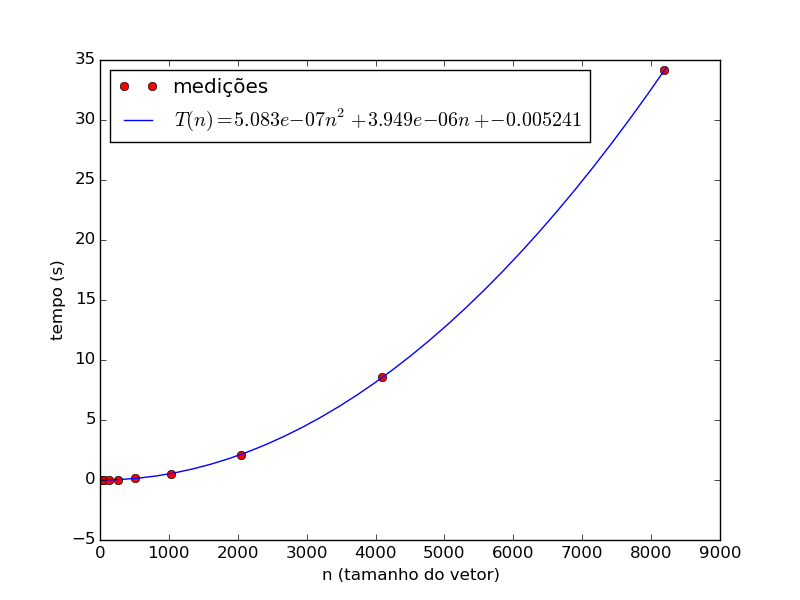
\includegraphics[scale=0.8]{../selectionsort/imagens/selectionsortAleatorio0.png}
\caption{A análise do grafico para $2^{32}$ segue abaixo para selectionsort}

Tendo a função $T(n) = 5.083\mathrm{e}-07*n^{2}+3.949\mathrm{e}-06*n-0.0052$ e para o $n =2^{32}$, $T(2^{32}) = 9.1376742 * 10^{301}$
\label{fig:selectionsortAleatorio0}
\end{figure}

\begin{figure}[ht]
\centering 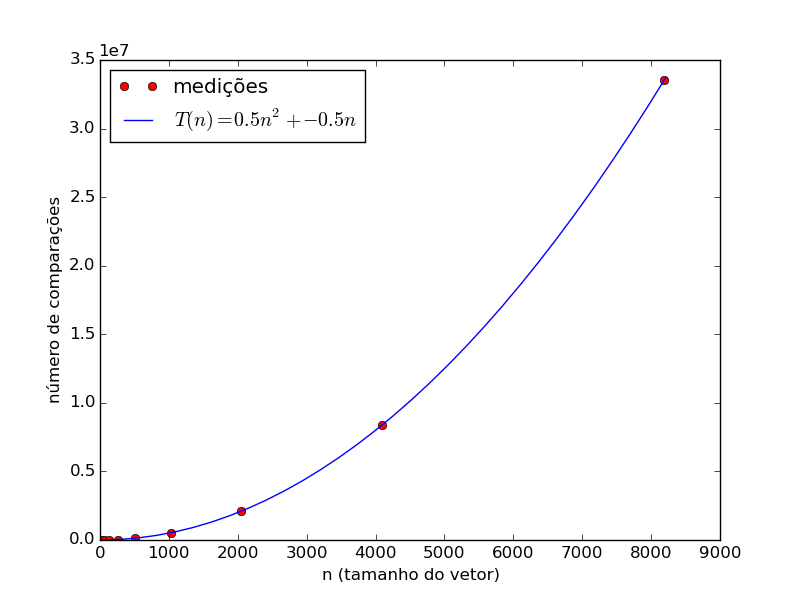
\includegraphics[scale=0.8]{../selectionsort/imagens/selectionsortAleatorio1.png}
\caption{A análise do grafico para $2^{32}$ segue abaixo para selectionsort}

Tendo a função $T(n) = 0.5*n^{2}-0.5*n$ e para o $n =2^{32}$, $T(2^{32}) =8.9884656 * 10^{307}$
\label{fig:selectionsortAleatorio1}
\end{figure}


\begin{table}[ht]
\centering
\begin{tabular}{rrr} \toprule
        n &    comparações &       tempo(s) \\ \midrule
      32  &            496 &      0.000648 \\
      64  &           2016 &      0.002277 \\
     128  &           8128 &      0.008596 \\
     256  &          32640 &      0.033311 \\
     512  &         130816 &      0.139917 \\
    1024  &         523776 &      0.522387 \\
    2048  &        2096128 &      1.987380 \\
    4096  &        8386560 &      8.685150 \\
    8192  &       33550336 &     34.369400 \\
\bottomrule\addlinespace
\end{tabular}
\caption{Tabela com vetor teste crescente: A linha te interesse analisada para este caso é a 15.}
\label{tab:selectionsortCrescente}
\end{table}


\begin{figure}[ht]
\centering 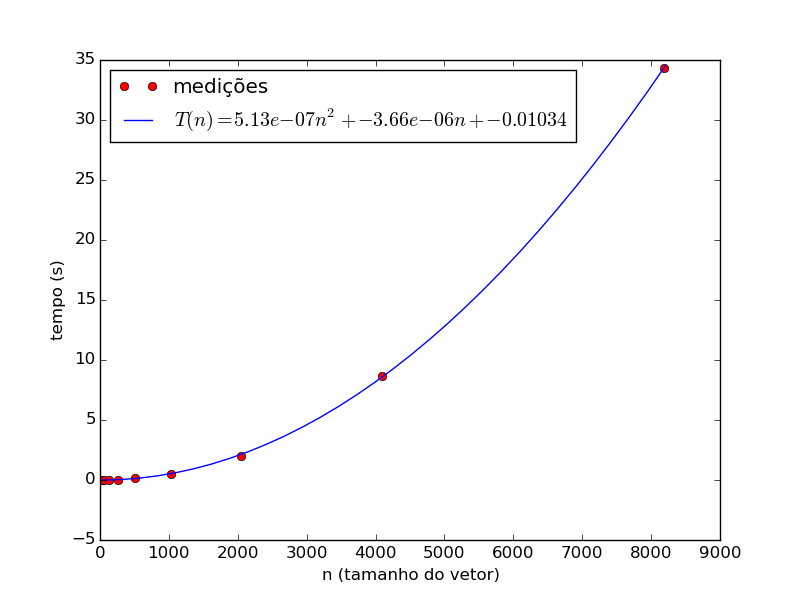
\includegraphics[scale=0.8]{../selectionsort/imagens/selectionsortCrescente0.png}
\caption{A análise do grafico para $2^{32}$ segue abaixo para selectionsort}

Tendo a função $T(n) = 5.13\mathrm{e}-07*n^{2}+3.66\mathrm{e}-06*n-0.001034$ e para o $n =2^{32}$, $T(2^{32}) = 9.222165 * 10^{301}$
\label{fig:selectionsortCrescente0}
\end{figure}

\begin{figure}[ht]
\centering 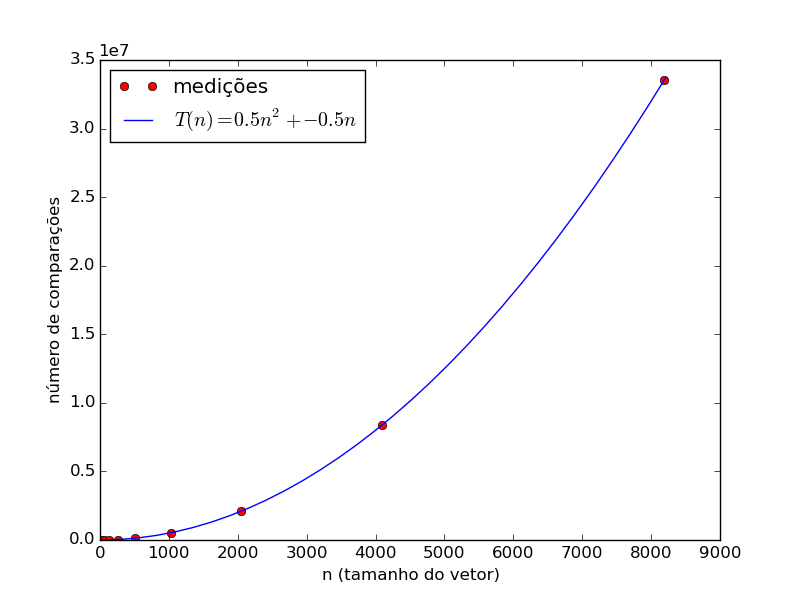
\includegraphics[scale=0.8]{../selectionsort/imagens/selectionsortCrescente1.png}
\caption{A análise do grafico para $2^{32}$ segue abaixo para selectionsort}

Tendo a função $T(n) = 0.5*n^{2}-0.5*n$ e para o $n =2^{32}$, $T(2^{32}) =8.9884656 * 10^{307}$
\label{fig:selectionsortCrescente1}
\end{figure}


\begin{table}[ht]
\centering
\begin{tabular}{rrr} \toprule
        n &    comparações &       tempo(s) \\ \midrule
      32  &            496 &      0.000672 \\
      64  &           2016 &      0.002618 \\
     128  &           8128 &      0.010014 \\
     256  &          32640 &      0.037622 \\
     512  &         130816 &      0.150541 \\
    1024  &         523776 &      0.604606 \\
    2048  &        2096128 &      2.596550 \\
    4096  &        8386560 &      9.657080 \\
    8192  &       33550336 &     34.009200 \\
\bottomrule\addlinespace
\end{tabular}
\caption{Tabela com vetor teste decrescente: A linha te interesse analisada para este caso é a 15.}
\label{tab:selectionsortDecrescente}
\end{table}


\begin{figure}[ht]
\centering 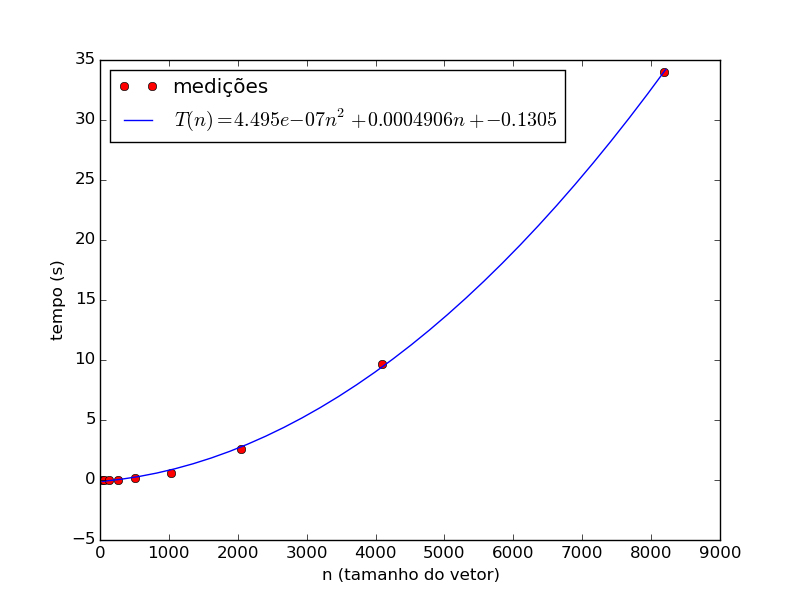
\includegraphics[scale=0.8]{../selectionsort/imagens/selectionsortDecrescente0.png}
\caption{A análise do grafico para $2^{32}$ segue abaixo para selectionsort}

Tendo a função $T(n) = 4.495\mathrm{e}-07*n^{2}+0.00049*n+0.1305$ e para o $n =2^{32}$, $T(2^{32}) = 8.0806306 * 10^{301}$
\label{fig:selectionsortDecrescente0}
\end{figure}

\begin{figure}[ht]
\centering 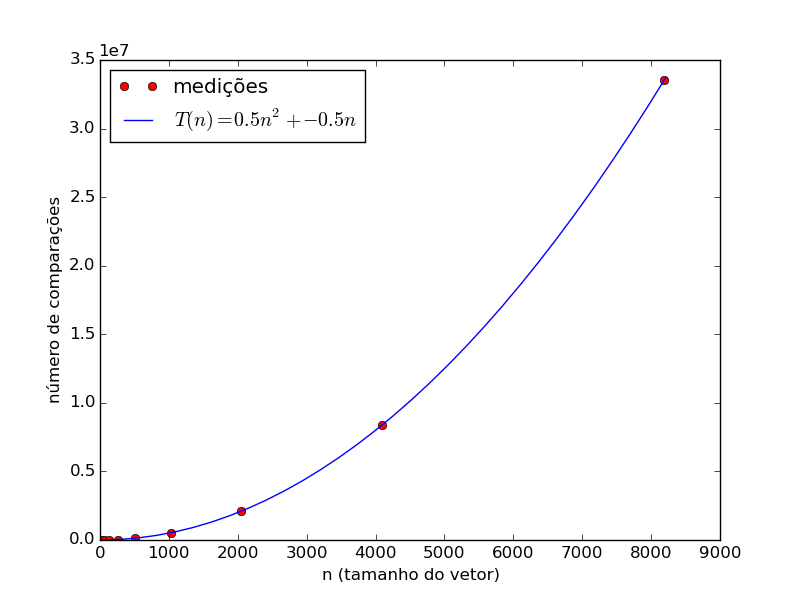
\includegraphics[scale=0.8]{../selectionsort/imagens/selectionsortDecrescente1.png}
\caption{A análise do grafico para $2^{32}$ segue abaixo para selectionsort}

Tendo a função $T(n) = 0.5*n^{2}-0.5*n$ e para o $n =2^{32}$, $T(2^{32}) =8.9884656 * 10^{307}$
\label{fig:selectionsortDecrescente1}
\end{figure}


\begin{table}[ht]
\centering
\begin{tabular}{rrr} \toprule
        n &    comparações &       tempo(s) \\ \midrule
      32  &            496 &      0.000613 \\
      64  &           2016 &      0.002308 \\
     128  &           8128 &      0.008188 \\
     256  &          32640 &      0.033693 \\
     512  &         130816 &      0.129137 \\
    1024  &         523776 &      0.579641 \\
    2048  &        2096128 &      1.999810 \\
    4096  &        8386560 &      9.121400 \\
    8192  &       33550336 &     32.989500 \\
\bottomrule\addlinespace
\end{tabular}
\caption{Tabela com vetor teste quase crescente 10\%: A linha te interesse analisada para este caso é a 15.}
\label{tab:selectionsortQuaseCresc10}
\end{table}


\begin{figure}[ht]
\centering 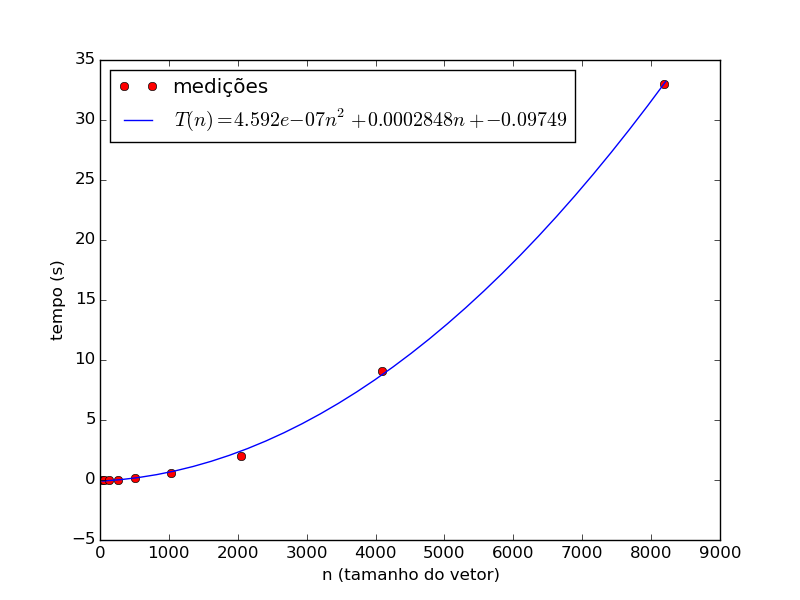
\includegraphics[scale=0.8]{../selectionsort/imagens/selectionsortQuaseCresc100.png}
\caption{A análise do grafico para $2^{32}$ segue abaixo para selectionsort}

Tendo a função $T(n) = 4.592\mathrm{e}-07*n^{2}+0.000284*n-0.09749$ e para o $n =2^{32}$, $T(2^{32}) = 8.25501*10^{301}$
\label{fig:selectionsortQuaseCresc100}
\end{figure}

\begin{figure}[ht]
\centering 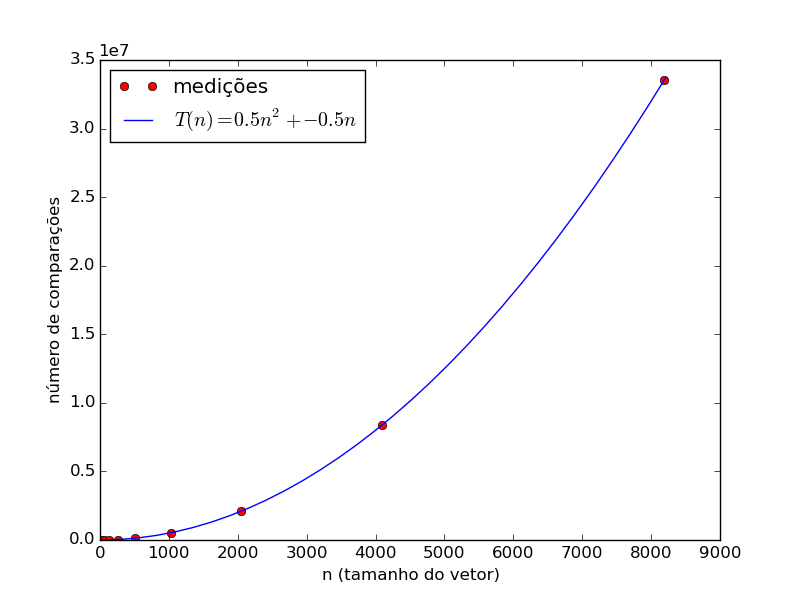
\includegraphics[scale=0.8]{../selectionsort/imagens/selectionsortQuaseCresc101.png}
\caption{A análise do grafico para $2^{32}$ segue abaixo para selectionsort}

Tendo a função $T(n) = 0.5*n^{2}-0.5*n$ e para o $n =2^{32}$, $T(2^{32}) =8.9884656 * 10^{307}$
\label{fig:selectionsortQuaseCresc101}
\end{figure}


\begin{table}[ht]
\centering
\begin{tabular}{rrr} \toprule
        n &    comparações &       tempo(s) \\ \midrule
      32  &            496 &      0.000627 \\
      64  &           2016 &      0.002248 \\
     128  &           8128 &      0.009107 \\
     256  &          32640 &      0.034544 \\
     512  &         130816 &      0.128516 \\
    1024  &         523776 &      0.526562 \\
    2048  &        2096128 &      2.038870 \\
    4096  &        8386560 &      9.178640 \\
    8192  &       33550336 &     32.969100 \\
\bottomrule\addlinespace
\end{tabular}
\caption{Tabela com vetor teste quase crescente 20\%: A linha te interesse analisada para este caso é a 15.}
\label{tab:selectionsortQuaseCresc20}
\end{table}


\begin{figure}[ht]
\centering 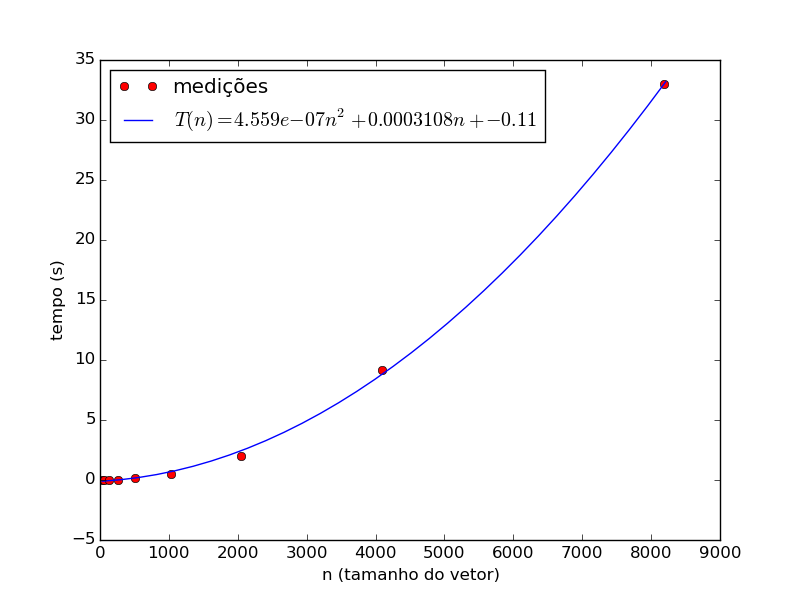
\includegraphics[scale=0.8]{../selectionsort/imagens/selectionsortQuaseCresc200.png}
\caption{A análise do grafico para $2^{32}$ segue abaixo para selectionsort}

Tendo a função $T(n) = 4.559\mathrm{e}-07*n^{2}+0.0003108*n-0.11$ e para o $n =2^{32}$, $T(2^{32}) = 8.19568*10^{301}$
\label{fig:selectionsortQuaseCresc200}
\end{figure}

\begin{figure}[ht]
\centering 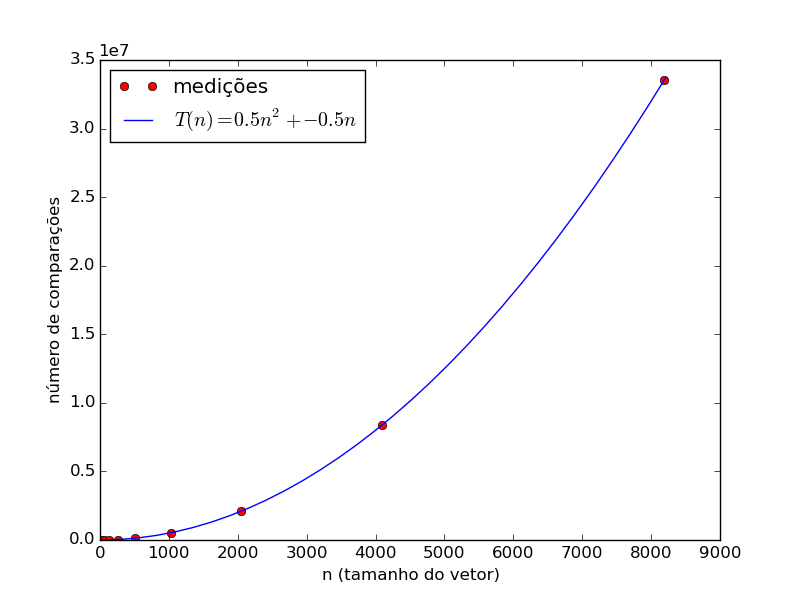
\includegraphics[scale=0.8]{../selectionsort/imagens/selectionsortQuaseCresc201.png}
\caption{A análise do grafico para $2^{32}$ segue abaixo para selectionsort}

Tendo a função $T(n) = 0.5*n^{2}-0.5*n$ e para o $n =2^{32}$, $T(2^{32}) =8.9884656 * 10^{307}$
\label{fig:selectionsortQuaseCresc201}
\end{figure}

\clearpage
\begin{table}[ht]
\centering
\begin{tabular}{rrr} \toprule
        n &    comparações &       tempo(s) \\ \midrule
      32  &            496 &      0.000576 \\
      64  &           2016 &      0.002319 \\
     128  &           8128 &      0.008653 \\
     256  &          32640 &      0.033483 \\
     512  &         130816 &      0.131007 \\
    1024  &         523776 &      0.541596 \\
    2048  &        2096128 &      2.069160 \\
    4096  &        8386560 &      8.934160 \\
    8192  &       33550336 &     34.025600 \\
\bottomrule\addlinespace
\end{tabular}
\caption{Tabela com vetor teste quase crescente 30\%: A linha te interesse analisada para este caso é a 15.}
\label{tab:selectionsortQuaseCresc30}
\end{table}


\begin{figure}[ht]
\centering 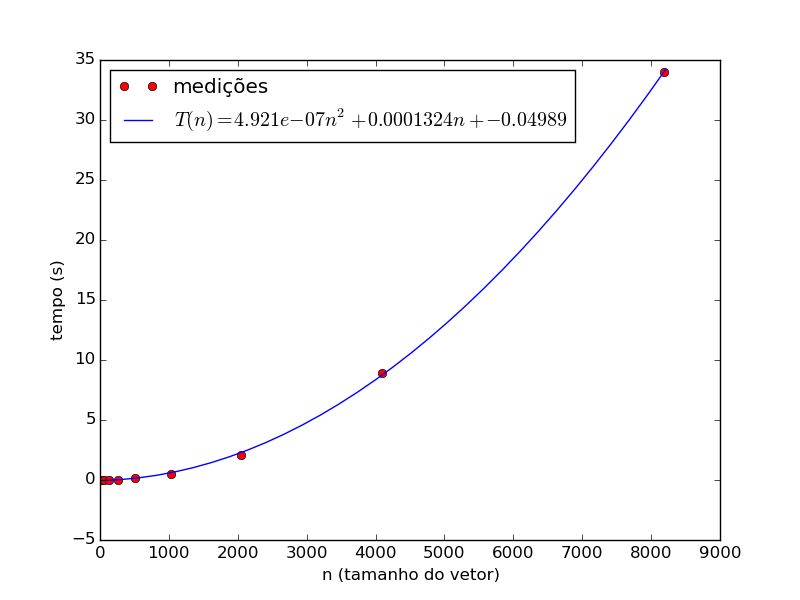
\includegraphics[scale=0.8]{../selectionsort/imagens/selectionsortQuaseCresc300.png}
\caption{A análise do grafico para $2^{32}$ segue abaixo para selectionsort}

Tendo a função $T(n) = 4.921\mathrm{e}-07*n^{2}+0.0001324*n-0.04989$ e para o $n =2^{32}$, $T(2^{32}) = 8.84645*10^{301}$
\label{fig:selectionsortQuaseCresc300}
\end{figure}

\begin{figure}[ht]
\centering 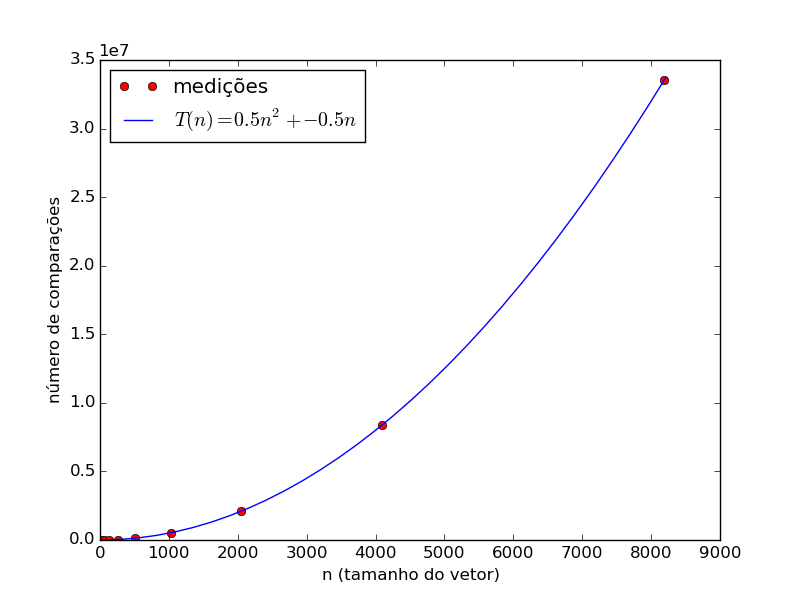
\includegraphics[scale=0.8]{../selectionsort/imagens/selectionsortQuaseCresc301.png}
\caption{A análise do grafico para $2^{32}$ segue abaixo para selectionsort}

Tendo a função $T(n) = 0.5*n^{2}-0.5*n$ e para o $n =2^{32}$, $T(2^{32}) =8.9884656 * 10^{307}$
\label{fig:selectionsortQuaseCresc301}
\end{figure}


\begin{table}[ht]
\centering
\begin{tabular}{rrr} \toprule
        n &    comparações &       tempo(s) \\ \midrule
      32  &            496 &      0.000602 \\
      64  &           2016 &      0.002394 \\
     128  &           8128 &      0.008284 \\
     256  &          32640 &      0.034522 \\
     512  &         130816 &      0.128441 \\
    1024  &         523776 &      0.520919 \\
    2048  &        2096128 &      2.154260 \\
    4096  &        8386560 &      8.764070 \\
    8192  &       33550336 &     34.113300 \\
\bottomrule\addlinespace
\end{tabular}
\caption{Tabela com vetor teste quase crescente 40\%: A linha te interesse analisada para este caso é a 15.}
\label{tab:selectionsortQuaseCresc40}
\end{table}


\begin{figure}[ht]
\centering 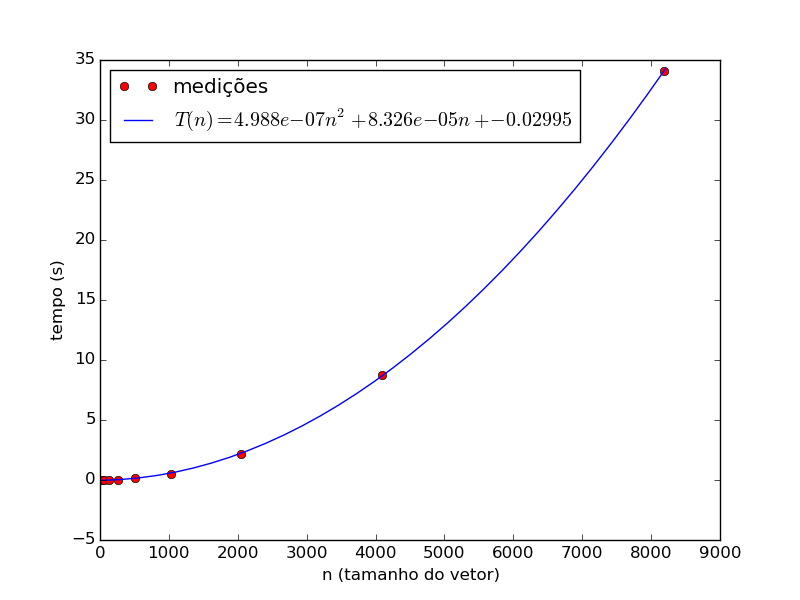
\includegraphics[scale=0.8]{../selectionsort/imagens/selectionsortQuaseCresc400.png}
\caption{A análise do grafico para $2^{32}$ segue abaixo para selectionsort}

Tendo a função $T(n) = 4.988\mathrm{e}-07*n^{2}+8.326\mathrm{e}-5*n-0.02995$ e para o $n =2^{32}$, $T(2^{32}) = 8.96689*10^{301}$
\label{fig:selectionsortQuaseCresc300}
\label{fig:selectionsortQuaseCresc400}
\end{figure}

\begin{figure}[ht]
\centering 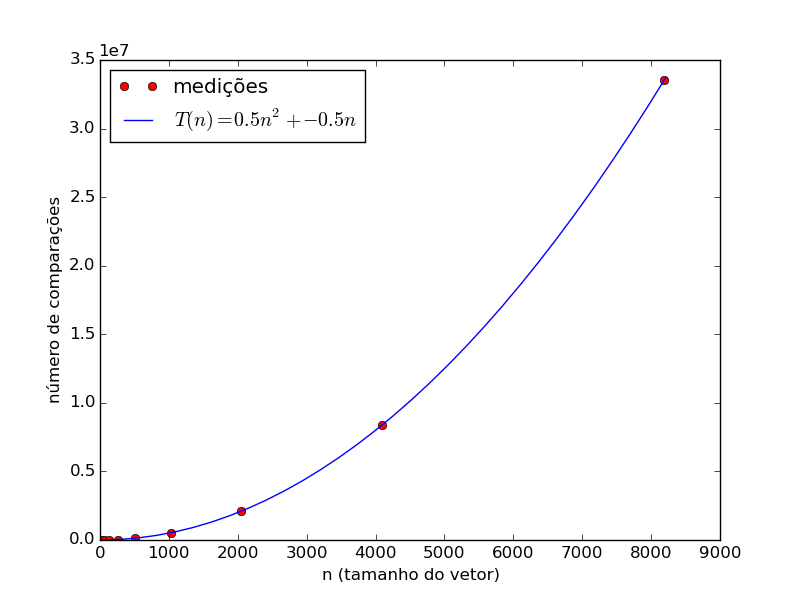
\includegraphics[scale=0.8]{../selectionsort/imagens/selectionsortQuaseCresc401.png}
\caption{A análise do grafico para $2^{32}$ segue abaixo para selectionsort}

Tendo a função $T(n) = 0.5*n^{2}-0.5*n$ e para o $n =2^{32}$, $T(2^{32}) =8.9884656 * 10^{307}$
\label{fig:selectionsortQuaseCresc401}
\end{figure}


\begin{table}[ht]
\centering
\begin{tabular}{rrr} \toprule
        n &    comparações &       tempo(s) \\ \midrule
      32  &            496 &      0.000622 \\
      64  &           2016 &      0.002407 \\
     128  &           8128 &      0.008500 \\
     256  &          32640 &      0.036190 \\
     512  &         130816 &      0.140001 \\
    1024  &         523776 &      0.573178 \\
    2048  &        2096128 &      2.058500 \\
    4096  &        8386560 &      9.339260 \\
    8192  &       33550336 &     31.402100 \\
\bottomrule\addlinespace
\end{tabular}
\caption{Tabela com vetor teste quase crescente 50\%: A linha te interesse analisada para este caso é a 15.}
\label{tab:selectionsortQuaseCresc50}
\end{table}


\begin{figure}[ht]
\centering 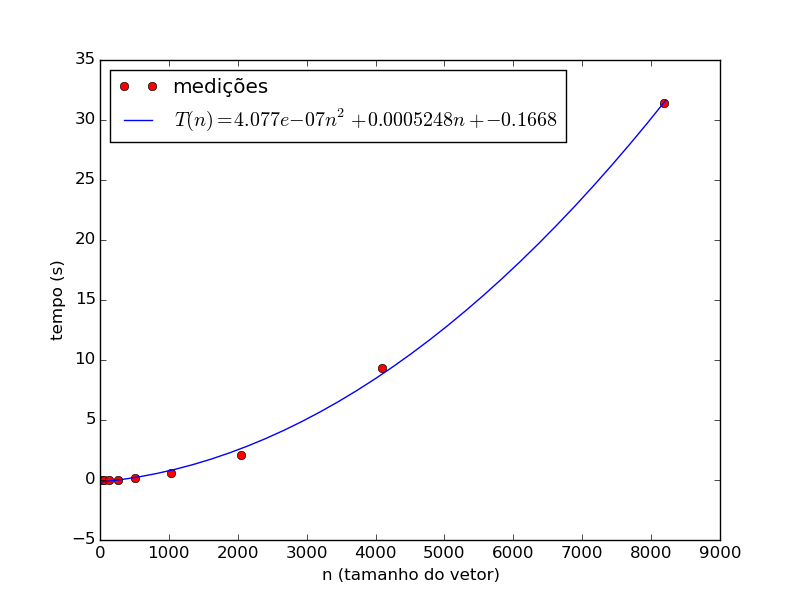
\includegraphics[scale=0.8]{../selectionsort/imagens/selectionsortQuaseCresc500.png}
\caption{A análise do grafico para $2^{32}$ segue abaixo para selectionsort}

Tendo a função $T(n) = 4.077\mathrm{e}-07*n^{2}+0.0005248*n-0.1668$ e para o $n =2^{32}$, $T(2^{32}) = 7.32919*10^{301}$
\label{fig:selectionsortQuaseCresc500}
\end{figure}

\begin{figure}[ht]
\centering 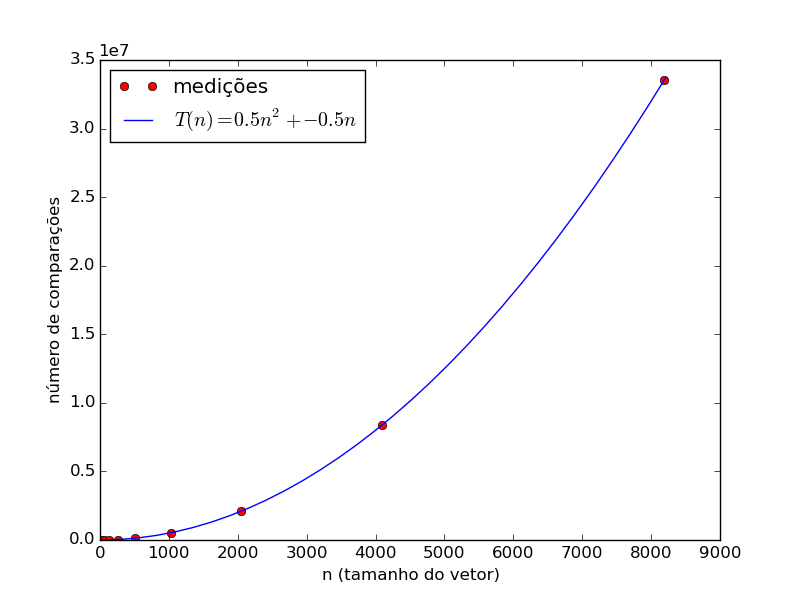
\includegraphics[scale=0.8]{../selectionsort/imagens/selectionsortQuaseCresc501.png}
\caption{A análise do grafico para $2^{32}$ segue abaixo para selectionsort}

Tendo a função $T(n) = 0.5*n^{2}-0.5*n$ e para o $n =2^{32}$, $T(2^{32}) =8.9884656 * 10^{307}$
\label{fig:selectionsortQuaseCresc501}
\end{figure}


\begin{table}[ht]
\centering
\begin{tabular}{rrr} \toprule
        n &    comparações &       tempo(s) \\ \midrule
      32  &            496 &      0.000708 \\
      64  &           2016 &      0.002590 \\
     128  &           8128 &      0.009378 \\
     256  &          32640 &      0.038826 \\
     512  &         130816 &      0.155937 \\
    1024  &         523776 &      0.615690 \\
    2048  &        2096128 &      2.513880 \\
    4096  &        8386560 &      9.210180 \\
    8192  &       33550336 &     34.747800 \\
\bottomrule\addlinespace
\end{tabular}
\caption{Tabela com vetor teste quase decrescente 10\%: A linha te interesse analisada para este caso é a 15.}
\label{tab:selectionsortQuaseDecresc10}
\end{table}


\begin{figure}[ht]
\centering 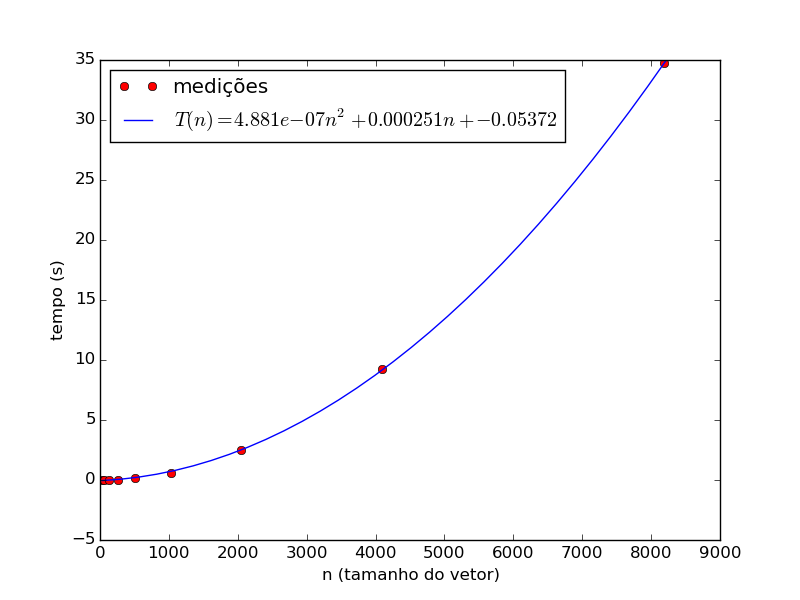
\includegraphics[scale=0.8]{../selectionsort/imagens/selectionsortQuaseDecresc100.png}
\caption{A análise do grafico para $2^{32}$ segue abaixo para selectionsort}

Tendo a função $T(n) = 4.881\mathrm{e}-07*n^{2}+0.000251*n-0.05372$ e para o $n =2^{32}$, $T(2^{32}) = 8.77454*10^{301}$
\label{fig:selectionsortQuaseDecresc100}
\end{figure}

\begin{figure}[ht]
\centering 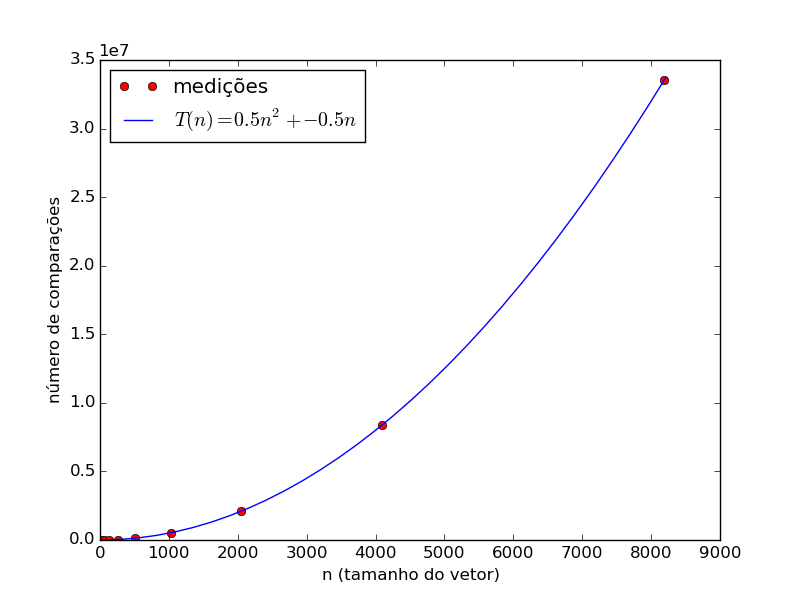
\includegraphics[scale=0.8]{../selectionsort/imagens/selectionsortQuaseDecresc101.png}
\\caption{A análise do grafico para $2^{32}$ segue abaixo para selectionsort}

Tendo a função $T(n) = 0.5*n^{2}-0.5*n$ e para o $n =2^{32}$, $T(2^{32}) =8.9884656 * 10^{307}$
\label{fig:selectionsortQuaseDecresc101}
\end{figure}


\begin{table}[ht]
\centering
\begin{tabular}{rrr} \toprule
        n &    comparações &       tempo(s) \\ \midrule
      32  &            496 &      0.000719 \\
      64  &           2016 &      0.002510 \\
     128  &           8128 &      0.008998 \\
     256  &          32640 &      0.038053 \\
     512  &         130816 &      0.136999 \\
    1024  &         523776 &      0.613878 \\
    2048  &        2096128 &      2.546130 \\
    4096  &        8386560 &      9.400370 \\
    8192  &       33550336 &     33.744400 \\
\bottomrule\addlinespace
\end{tabular}
\caption{Tabela com vetor teste quase decrescente 20\%: A linha te interesse analisada para este caso é a 15}
\label{tab:selectionsortQuaseDecresc20}
\end{table}


\begin{figure}[ht]
\centering 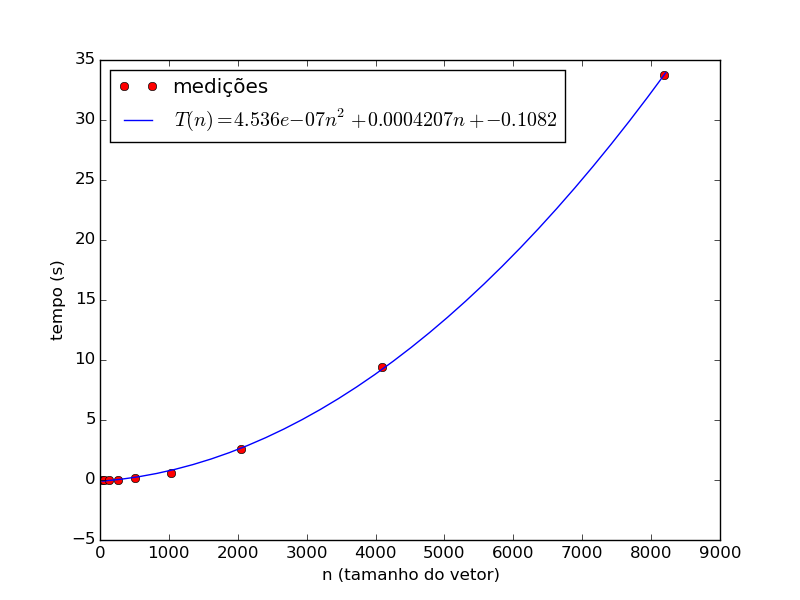
\includegraphics[scale=0.8]{../selectionsort/imagens/selectionsortQuaseDecresc200.png}
\caption{A análise do grafico para $2^{32}$ segue abaixo para selectionsort}

Tendo a função $T(n) = 4.536\mathrm{e}-07*n^{2}+0.0004207*n-0.1082$ e para o $n =2^{32}$, $T(2^{32}) = 8.15434*10^{301}$
\label{fig:selectionsortQuaseDecresc200}
\end{figure}

\begin{figure}[ht]
\centering 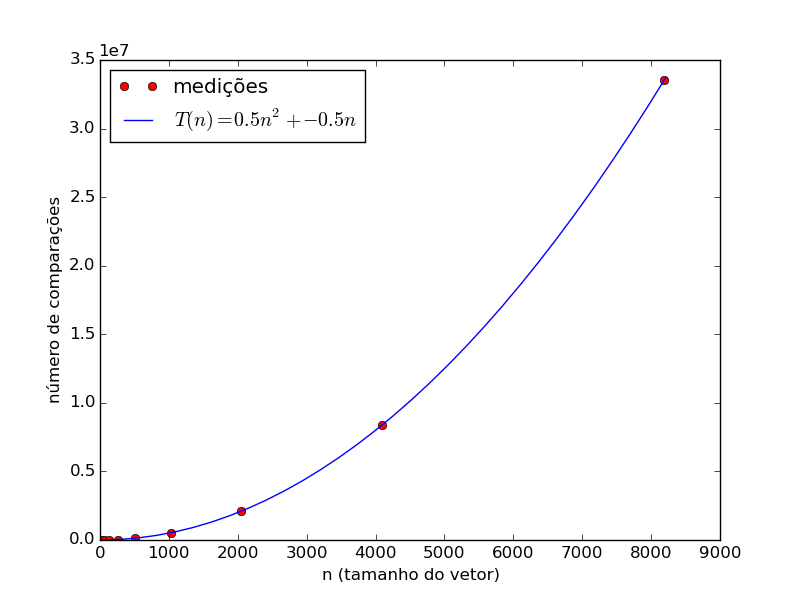
\includegraphics[scale=0.8]{../selectionsort/imagens/selectionsortQuaseDecresc201.png}
\caption{A análise do grafico para $2^{32}$ segue abaixo para selectionsort}

Tendo a função $T(n) = 0.5*n^{2}-0.5*n$ e para o $n =2^{32}$, $T(2^{32}) =8.9884656 * 10^{307}$
\label{fig:selectionsortQuaseDecresc201}
\end{figure}

\clearpage
\begin{table}[ht]
\centering
\begin{tabular}{rrr} \toprule
        n &    comparações &       tempo(s) \\ \midrule
      32  &            496 &      0.000684 \\
      64  &           2016 &      0.002557 \\
     128  &           8128 &      0.009644 \\
     256  &          32640 &      0.038745 \\
     512  &         130816 &      0.144655 \\
    1024  &         523776 &      0.567072 \\
    2048  &        2096128 &      2.242760 \\
    4096  &        8386560 &      9.866570 \\
    8192  &       33550336 &     34.645600 \\
\bottomrule\addlinespace
\end{tabular}
\caption{Tabela com vetor teste quase decrescente 30\%: A linha te interesse analisada para este caso é a 15}
\label{tab:selectionsortQuaseDecresc30}
\end{table}


\begin{figure}[ht]
\centering 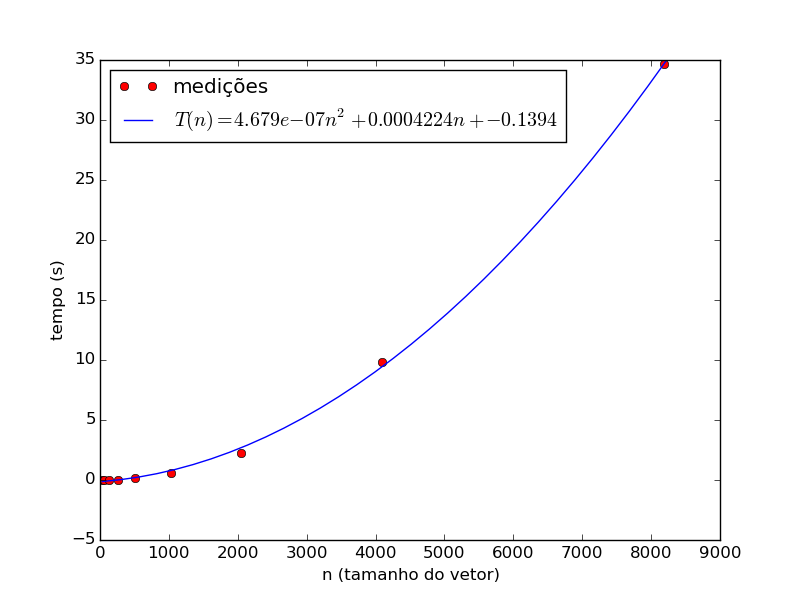
\includegraphics[scale=0.8]{../selectionsort/imagens/selectionsortQuaseDecresc300.png}
\caption{A análise do grafico para $2^{32}$ segue abaixo para selectionsort}

Tendo a função $T(n) = 4.679*n^{2}-07*n-0.1394$ e para o $n =2^{32}$, $T(2^{32}) =8.411406178020777*10^{308}$
\label{fig:selectionsortQuaseDecresc201}
\label{fig:selectionsortQuaseDecresc300}
\end{figure}

\begin{figure}[ht]
\centering 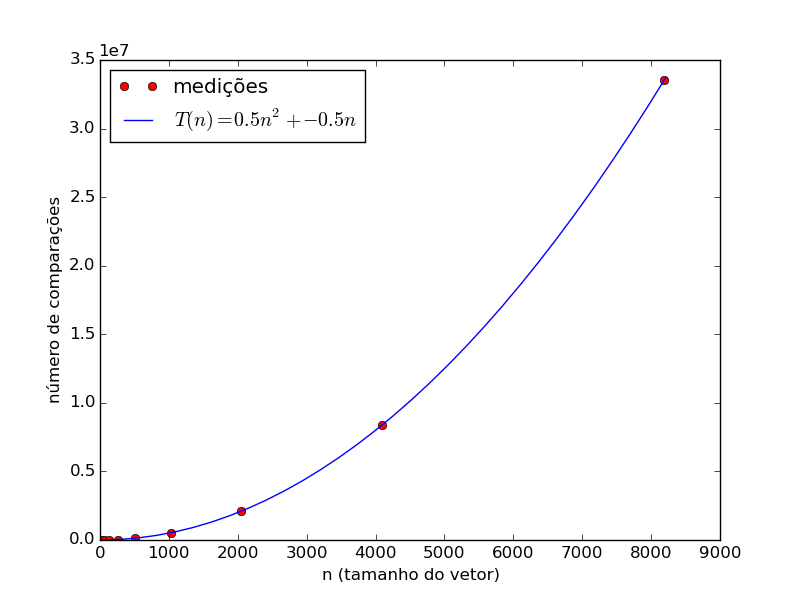
\includegraphics[scale=0.8]{../selectionsort/imagens/selectionsortQuaseDecresc301.png}
\caption{A análise do grafico para $2^{32}$ segue abaixo para selectionsort}

Tendo a função $T(n) = 0.5*n^{2}-0.5*n$ e para o $n =2^{32}$, $T(2^{32}) =8.9884656 * 10^{307}$
\label{fig:selectionsortQuaseDecresc301}
\end{figure}


\begin{table}[ht]
\centering
\begin{tabular}{rrr} \toprule
        n &    comparações &       tempo(s) \\ \midrule
      32  &            496 &      0.000655 \\
      64  &           2016 &      0.002451 \\
     128  &           8128 &      0.009061 \\
     256  &          32640 &      0.036720 \\
     512  &         130816 &      0.140110 \\
    1024  &         523776 &      0.625800 \\
    2048  &        2096128 &      2.254600 \\
    4096  &        8386560 &      8.999930 \\
    8192  &       33550336 &     35.220200 \\
\bottomrule\addlinespace
\end{tabular}
\caption{Tabela com vetor teste quase decrescente 40\%: A linha te interesse analisada para este caso é a 15}
\label{tab:selectionsortQuaseDecresc40}
\end{table}


\begin{figure}[ht]
\centering 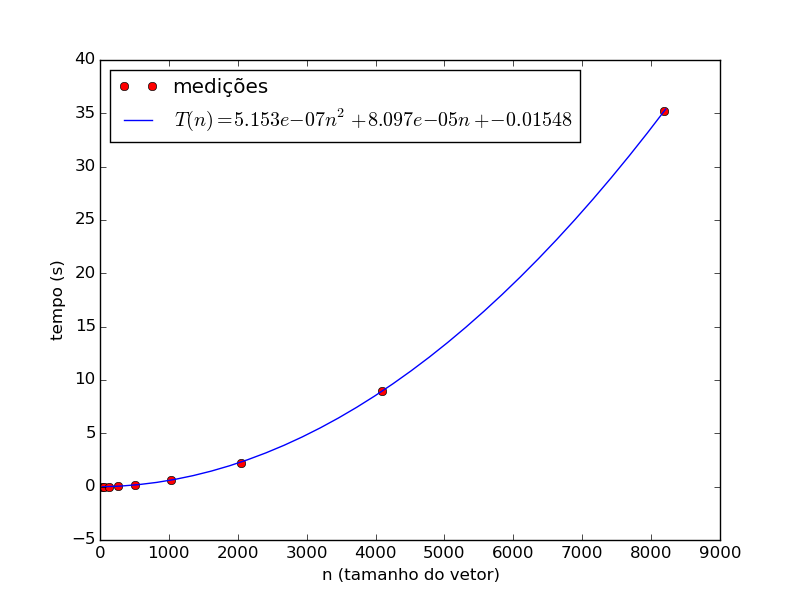
\includegraphics[scale=0.8]{../selectionsort/imagens/selectionsortQuaseDecresc400.png}
\caption{A análise do grafico para $2^{32}$ segue abaixo para selectionsort}

Tendo a função $T(n) = 5.153\mathrm{e}-07*n^{2}+8.097\mathrm{e}-5*n-0.01548$ e para o $n =2^{32}$, $T(2^{32}) =9.26351272 * 10^{301}$
\label{fig:selectionsortQuaseDecresc400}
\end{figure}

\begin{figure}[ht]
\centering 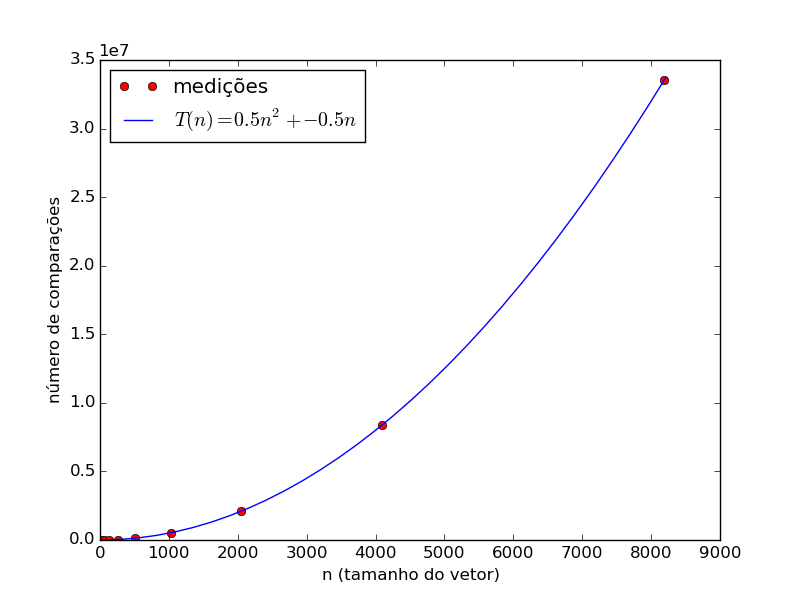
\includegraphics[scale=0.8]{../selectionsort/imagens/selectionsortQuaseDecresc401.png}
\caption{A análise do grafico para $2^{32}$ segue abaixo para selectionsort}

Tendo a função $T(n) = 0.5*n^{2}-0.5*n$ e para o $n =2^{32}$, $T(2^{32}) =8.9884656 * 10^{307}$
\label{fig:selectionsortQuaseDecresc401}
\end{figure}


\begin{table}[ht]
\centering
\begin{tabular}{rrr} \toprule
        n &    comparações &       tempo(s) \\ \midrule
      32  &            496 &      0.000679 \\
      64  &           2016 &      0.002268 \\
     128  &           8128 &      0.009045 \\
     256  &          32640 &      0.034093 \\
     512  &         130816 &      0.141664 \\
    1024  &         523776 &      0.531386 \\
    2048  &        2096128 &      2.157350 \\
    4096  &        8386560 &      8.908460 \\
    8192  &       33550336 &     35.002700 \\
\bottomrule\addlinespace
\end{tabular}
\caption{Tabela com vetor teste quase decrescente 50\%: A linha te interesse analisada para este caso é a 15}
\label{tab:selectionsortQuaseDecresc50}
\end{table}


\begin{figure}[ht]
\centering 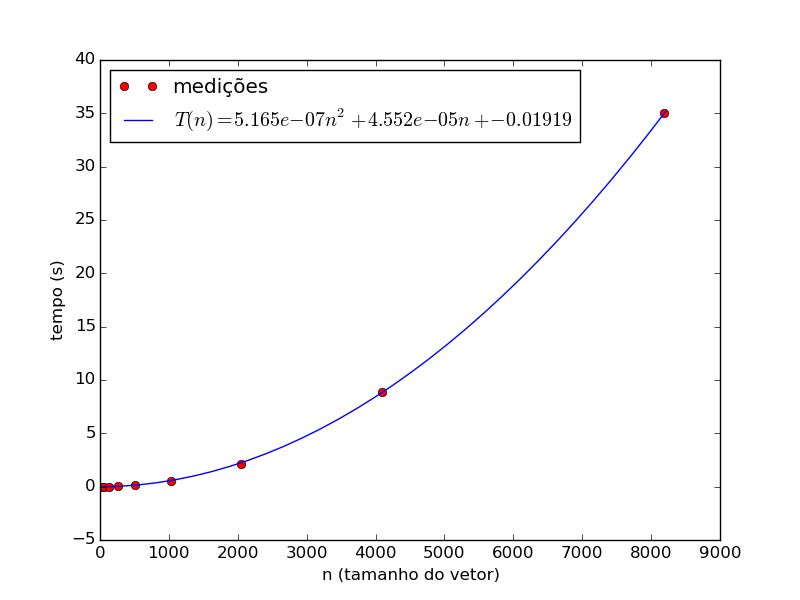
\includegraphics[scale=0.8]{../selectionsort/imagens/selectionsortQuaseDecresc500.png}
\caption{A análise do grafico para $2^{32}$ segue abaixo para selectionsort}

Tendo a função $T(n) = 5.165\mathrm{e}-07*n^{2}+4.552\mathrm{e}-5*n-0.01919$ e para o $n =2^{32}$, $T(2^{32}) =9.2850850415 * 10^{301}$
\label{fig:selectionsortQuaseDecresc500}
\end{figure}

\begin{figure}[ht]
\centering 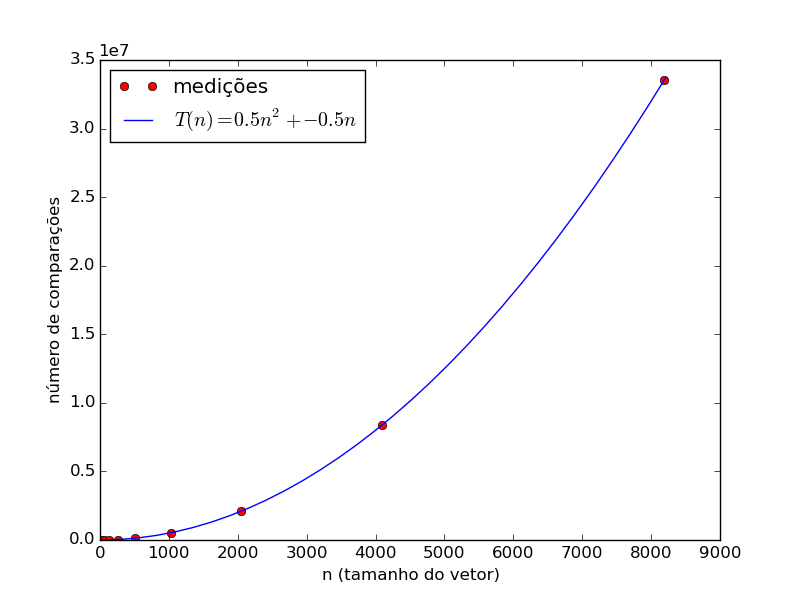
\includegraphics[scale=0.8]{../selectionsort/imagens/selectionsortQuaseDecresc501.png}
\caption{A análise do grafico para $2^{32}$ segue abaixo para selectionsort}

Tendo a função $T(n) = 0.5*n^{2}-0.5*n$ e para o $n =2^{32}$, $T(2^{32}) =8.9884656 * 10^{307}$
\label{fig:selectionsortQuaseDecresc501}
\end{figure}


\clearpage
\clearpage
\addcontentsline{toc}{part}{Apêndice}
\appendix

\chapter{Arquivo ../selectionsort/selectionsort.py \label{ap:selectionsort}}
\lstinputlisting[caption={../selectionsort/selectionsort.py \label{arq:selectionsort}}]{../selectionsort/selectionsort.py}

\chapter{Arquivo ../selectionsort/ensaio.py \label{ap:selectionsortensaio}}
\lstinputlisting[caption={../selectionsort/ensaio.py \label{arq:selectionsortensaio}}]{../selectionsort/ensaio.py}

\end{document}
